\documentclass[preview]{standalone}
\usepackage{pgfplots}
\usepgfplotslibrary{smithchart}
\pgfplotsset{compat=1.17}

\begin{document}
    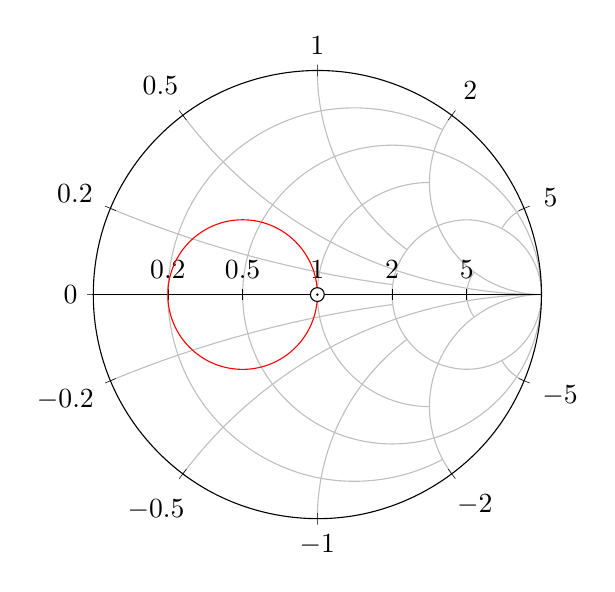
\begin{tikzpicture}
        \begin{smithchart}[
            show origin,]
        % % Reactance plot
        % \addplot[domain=0:90, samples=600, color=blue] {.5};

        % % Resistance plot - orange 
        % \addplot+[samples at={.5, .51,...,5},
        % smooth, color={orange},mark size=.2,line width=1](.5,x) ;

        % \addplot+[samples at={.5, .51,...,5},
        % smooth, color={green},mark size=.2,line width=1](x,.2) ;

        % Resistance plot - red 
        % \addplot+[samples at={-5, -4.99,...,5},
        % smooth, color={red},mark size=.2,line width=1] (.5,x) ;
        %% Unit circle
        \path[draw=red] (0.5,0) circle (.95cm);

        % \path[draw=red, thick] (-.5cm,0cm) circle [radius=.1cm];
            
        \end{smithchart}
    \end{tikzpicture}
\end{document}